\chapter{Design}
In this chapter, I aim to present two distinct designs for implementing
software-defined CPU modes. The primary approach under discussion involves the
integration of a single hardware supported CPU mode  that enables the definition
of additional modes in software. The difference to "Programmable Mode-based
Memory Isolation" is a more flexible approach. There is no more hierarchy between
modes and no hardware defined mode switch behavior. I will delve into the
specific hardware components that necessitate migration to software to support
this concept. Additionally, I will expound upon the methodology for defining and
storing modes while identifying the requisite new instructions to be
incorporated into the Instruction Set Architecture (ISA).\par
The second design I will explore introduces an additional core to our CPU,
selectively activated for mode switching, accounting, and CPU reconfiguration
purposes. This innovative design anticipates addressing potential performance
bottlenecks that may arise from executing mode handling on the same core. I will
explain which CPU components must be made accessible by this supplementary
core to ensure seamless functionality. Moreover, I will examine the feasibility
of incorporating elements from the extra mode design onto the supplementary CPU.  

\section{Mode Switch Mode}
This section will present the design of an additional mode, termed as the "Mode
Switch Mode," dedicated to managing mode switching and definitions within the
CPU architecture. The Mode Switch Mode serves as the sole mode defined by the
hardware, equipped with the capability to define other modes. It operates as a
programmable supervisor mode for mode creation and seamless transitions between
them, allowing software to freely define the target mode and actions during the
transition. This programmability enables dynamic mode management, entirely
controlled by software interventions.\par
To enable this functionality, specific alterations to the CPU architecture are
necessary. In Figure \ref{fig:msm_schema} you can see that there are two new
control and status registers added in. The interrupt and fault handling
mechanism where restructured and some new structures, the Mode-Lookaside-Buffer
and the Permission-Lookaside-Buffer where added to the MMU. To use some of this
changes new instruction have been added and the preexisting \texttt{mret} has
been altered. In the subsequent sections I will explain this changes in more detail.

\begin{figure}[h]
    \centering
    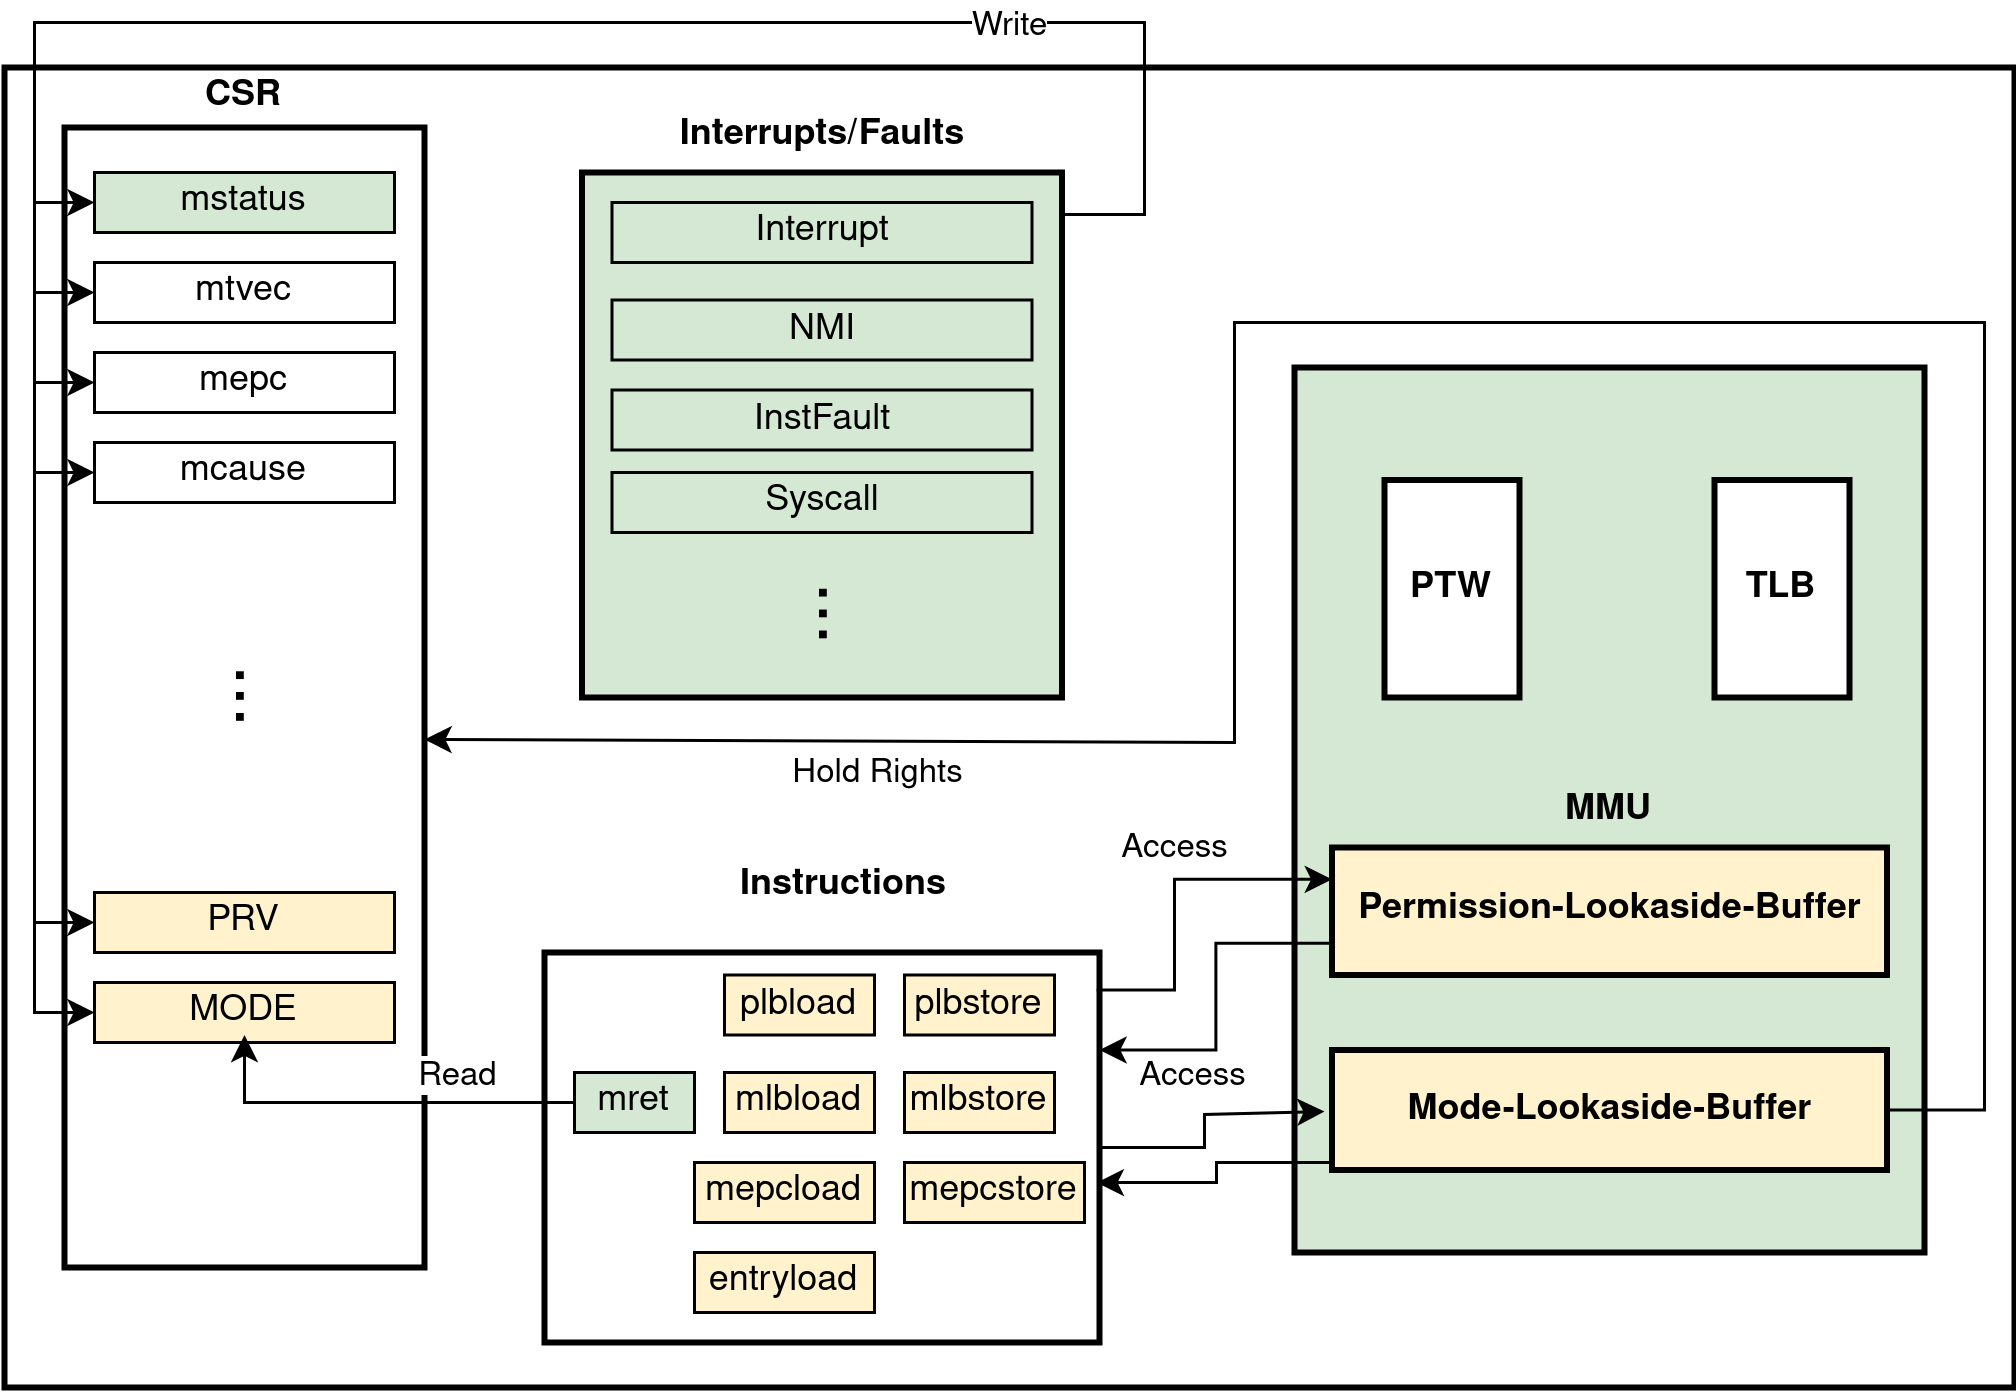
\includegraphics[width=1\textwidth]{MSM_schema}
    \captionsetup{justification=centering}
    \caption{Schema for the Mode Switch Mode}
            Yellow symbolizes elements that are newly added, green marks
            elements which were in the original Risc-V design and have now a
            slightly different design. 
    \label{fig:msm_schema}
\end{figure}

\subsection{Modes}
The first question to answer was how modes are defined. Should modes be
implicitly identified by the resources which are currently available or should
they be explicitly identified by an Id ? I decided to implement modes explicitly
because it seems easier to create a flexible design where modes can be created
and accounted during runtime with Ids instead of always keeping track which
resources are made available at the current time.\par
Another question is should this modes have a hierarchy or be completely free
standing. One could argue that a hierarchical approach makes sense to keep track
of which mode can destroy or create an other mode. Further it eases some
security checks regarding child calls, so that a mode can not call arbitrary
into an other mode as Von Elm describes it in his thesis. Figure \ref{fig:free_schema} shows what would
need to be done to change from a one mode to another with in a hierarchy. The
call to the parent would be implemented in hardware and therefore add some
implicit security. In a freestanding design such a jump to the parent also
happens. In this case the Mode Switch Mode can be seen as the parent mode where
arbitrary calls are not possible. So a free standing implementation of the
modes wouldn't change much of the behavior but adds more flexibility for the
Mode Switch Mode. Therefore I decided to use a free standing implementation of
modes.

\begin{figure}[h]
    \centering
    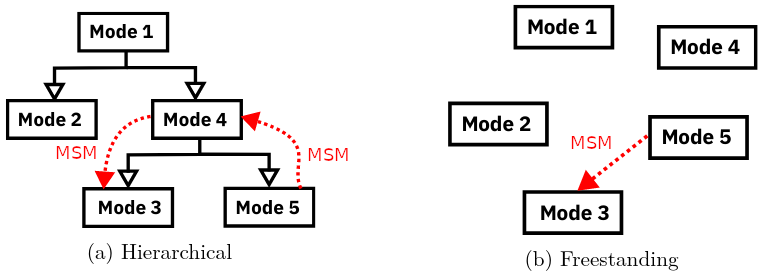
\includegraphics[width=1\textwidth]{free_vs_hier} 
    \captionsetup{justification=centering}
    \caption{Hierarchical and Free-standing mode switch}
            The red arrow denotes what it takes to change the mode. Every MSM
            shows when the Mode Switch Mode is entered. The Mode Switch Mode
            acts as a parent mode in the freestanding implementation where an
            arbitrary jump is not possible. It just enables a more flexible
            design of how to switch modes. A hierarchy where a jump is routed
            through a parent mode just increases the number of modes that are
            entered.
    \label{fig:free_schema}
\end{figure}

\subsection{Mode Accounting}
Following the introduction of modes, I want to show how modes are accounted in
efficient way. This is crucial because the mode restoration could otherwise impose a
significant overhead on the Mode Switch which should be as quick as possible.
Addressing this issue, Von Elm\cite{Cve} encountered a similar challenge and
devised a solution in his work. He proposed a Mode-Lookaside-Buffer(MLB)
architecture to store mode descriptor which hold all necessary information
about a modes state and access rights.\par
I decided to use the same infrastructure for this project. For this work I
created the following mode descriptor(see Fig.\ref{fig:mode_descriptor}) along
some special instructions for altering it which are only available in the Mode
Switch Mode. The first 64 bit of the mode
descriptor are for a entry point into the mode. This can be used to access a
mode if it has never been run before and has no current program counter or if
this mode has a handler routine which should be called on entering this mode. To
load the address from this field the \texttt{loadentry} instruction was created
to quickly load this address. There is no special write instruction to this
field, because once it is set it shouldn't be changed anymore. Because of this
the entry point field should be set on creation of a mode descriptor when it is
saved with the \texttt{mlbstore} instruction. The whole descriptor can be loaded
for later alteration with the \texttt{mlbload} instruction but this is a
performance heavy access because we now have one load and one store instruction.\par
The second 64 bit hold the program counter. This field can be used if a mode
should restart its execution at a certain point for example when it is
interrupted or made a system call after which it wants to reenter its own
control flow. Because this field can be written on every mode switch, there is
the \texttt{mepcstore} instruction which writes an address to the \texttt{EPC}
field of the mode descriptor. It can be restored with \texttt{mepcload}. The
handling which address should be loaded, either the entry point or the last
program counter, can be implemented in the mode switch mode by the systems
programmer.\par
The next 16 bit of the descriptor are the Id which is used to identify modes.
Because it should only be set on mode creation there are no special instructions
to read or write this field. It is mostly used in hardware to find check if a
mode has certain rights and to find a mode if a \texttt{mepcload} or an other of
the special instructions is used.\par
The next 3 bits are currently unused but could implement some interrupt
forwarding capability in the future. The last 45 bits are used to describe
access rights to the control and status registers. Due to its complexity this
topic will be discussed in the next section.

\begin{figure}[h]
    \centering
    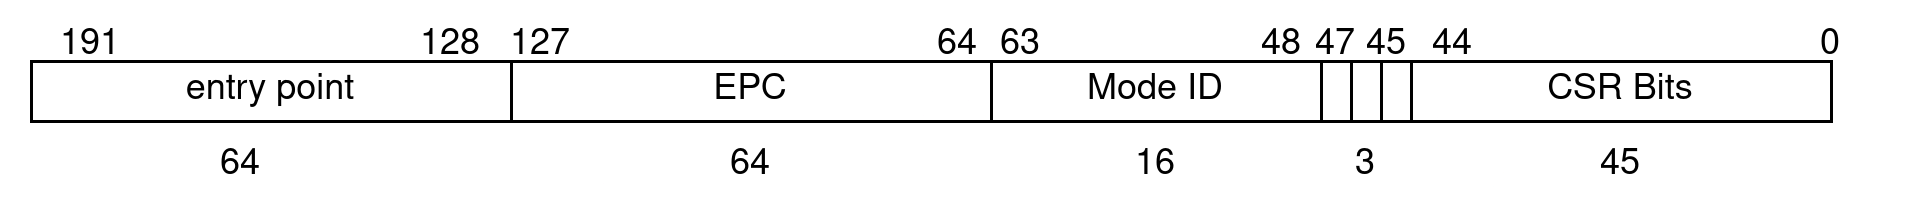
\includegraphics[width=\textwidth]{modeentry}
    \caption{Mode descriptor}
    \label{fig:mode_descriptor}
\end{figure}

\subsection{Control and Status Registers}
One of the core parts of mode isolation in RiscV are the control and status
registers. Some of them are only accessible in a certain mode. To give the full
control about mode creation this rights need to be dynamically changeable. This
is done with the last 45 bits of the mode descriptor. The bits represents the
access rights to the CSRs. If this bit is set a mode has read and write access
to this CSR. To reduce the amount of bits for all 119 CSRs some of them are
grouped together. This means from bit 44 till bit 2 they represent all CSRs from
top to bottom without the HPM und PMP registers because if a mode have access to
one of the HPM or PMP registers, it should have access to all of the HPM or PMP
registers. This means that bit 1 represents access to the HPM registers and bit
0 represents access to the PMP registers. In RiscV the CSRs are written with
special \texttt{csrr} instruction. On execute of this instructions a check is
run against the mode descriptor if this instruction is possible.\par
This check uses the \texttt{prv} CSR which holds the current mode to identify
against which descriptor should be checked. The access rights of \texttt{prv}
can not be changed and it is only writeable by the hardware. This
CSR was newly introduced to hold the mode id of the currently running mode.
As you can see in Figure \ref{fig:msm_schema} another new CSR is the \texttt{mode} field which
holds the previous mode while the Mode Switch Mode is entered and holds the
target mode when the Mode Switch Mode is left.\par
The only way to change the \texttt{prv} CSR is the \texttt{mret} instruction. It
is only available to the Mode Switch Mode and is used to change back from the
Mode Switch Mode to any target mode. Therefore the \texttt{prv} register is set
to the value of the \texttt{mode} register effectively changing the mode of the
CPU. During the \texttt{mret} the interrupt enable bit in the \texttt{mstatus}
is not changed enable the programmer to allow mode switch with disabled
interrupt for example when entering an interrupt handler in a special interrupt
handling mode. The program counter for the entered mode is loaded from the
\texttt{mepc} register.

\subsection{Traps and Mode Change}
After detailing the methods to access and manipulate different CPU states and
modes, I want to explain how the transition into the Mode Switch Mode
occurs and which information is preserved during this process.\par
Every trap, encompassing interrupts, faults, or syscalls, redirects control flow
into the Mode Switch Mode. During this transition, interrupts are disabled,
ensuring entry into the Mode Switch Mode with interrupts turned off. The current
program counter is preserved within the \texttt{mepc} register, while the program counter
is set to the value contained in the \texttt{mtvec} register. The mode which we
are leaving is written to the \texttt{mode} register. All other registers treated like in
an normal RiscV implementation.\par
\vspace{12pt}
Having explained the essential building blocks necessary for a
simple transition from the Mode Switch Mode to another mode, I'll provide a
quick overview of how the mode descriptor and the new CSRs work together.\par
Upon arrival at the Mode Switch Mode, the program counter for the previous mode
is loaded from the \texttt{mepc} register and then stored via the
\texttt{mepcstore} instruction into the mode descriptor. The mode Id for this
descriptor can be retrieved from the \texttt{mode} register. Subsequently, the Mode Switch Mode determines
the correct mode to switch to. Once this mode is identified, the address where
the new mode starts can be loaded, either with \texttt{mepcload} or
\texttt{entryload} from the according mode descriptor field. The loaded address
is then stored into the \texttt{mepc} register.\par 
Concurrently, the \texttt{mode} register is updated with the ID of this newly
targeted mode. If the new mode is intended to start with interrupts enabled,
this setting should be enabled at this stage by the Mode Switch Mode code.
Finally, invoking the \texttt{mret} instruction effectuates the mode change.
These outlined steps constitute the minimal procedural actions when
transitioning from one mode to another. However, additional steps, such as
saving specific registers  can also be incorporated.\par
Regarding the initial configuration, upon processor boot-up, the system
starts in the Mode Switch Mode, allowing for essential configurations. The
\texttt{mtvec} register should be set to point to the handler of the Mode Switch Mode.

\subsection{Memory Protection}
An essential aspect of modes is memory protection, particularly in the context
of memory virtualization. As the number of modes increases, the traditional
paging approach faces limitations. The conventional paging system encounters
challenges in efficiently storing access information for each mode within the
page table entry, especially with a rapidly escalating number of permission bit entries even
for a relatively small number of modes. A proposed solution is to split the
accounting and permission handling parts, typically executed simultaneously.
This separation is due to the inherent strength of paging in accounting for
memory locations with uniform sizes but lacks efficiency in verifying access
rights for irregularly shaped memory segments composed of multiple pages (for
further insights, refer to Chapter \ref{chap:mem_perm}).\par
Addressing this challenge, Von Elm et al.\cite{Cve} have already provided a solution. He
leverage the paging method for accounting purposes, as the page table walk
offers the most compact footprint to record the relationship between physical
and virtual memory. For the access rights control aspect, they employ a
segmentation-based approach. Here, memory locations starting from a designated
start address and ending at an address calculated by an offset from the start
address possess certain access rights. The page-permission bits will remain
as-is. The permissions assigned to a memory address in this setup represent the
minimum of the permissions granted by both the paging and mode systems. In cases
where the mode system designates read and write permissions for an address,
while the page table specifies read and execute permissions, the address will
only be accessible for reading. To define these memory locations, a segment
descriptor (illustrated in Fig. \ref{fig:plb_descriptor}) is formulated,
encompassing details such as the start address, offset, and permission bits.\par

\begin{figure}[h]
    \centering
    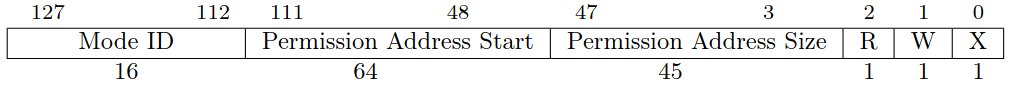
\includegraphics[width=\textwidth]{plb}
    \caption{PLB descriptor}
    \label{fig:plb_descriptor}
\end{figure}

To optimize performance, this descriptor is loaded into the
Permission-Lookaside-Buffer (PLB), allowing the Memory Management Unit (MMU) to
efficiently fetch information regarding access rights during the page table
walk. Programmers can populate this buffer using the \texttt{plbstore} and \texttt{plbload}
instructions within the Mode Switch Mode. The segmentation layer always needs to be
configured on top of the paging layer. Given that the primary focus of this
work isn't solely on memory protection, I integrated this working
solution into my design to address this crucial aspect.

\section{Control Core}
This section explains the second approach involving an additional core
dedicated to managing all mode switch activities. Named the Control Core, this
entity exists alongside the CPU as an independent unit with its dedicated
memory(see Fig. \ref{fig:cc_schema}). Conceptually, it resembles an accelerator
where the CPU delegates all mode switch responsibilities. The Control Core
encompasses all functionalities offered by the Mode Switch Mode.\par
The rationale behind this approach lies in the anticipation of performance
benefits by offloading mode switch handling onto a secondary core equipped with
its own registers. If the Mode Switch Mode runs on the same CPU whenever a this
mode is entered and want to use some registers, the used registers need to be
saved and restored before we are leaving this mode. As the Mode Switch Mode is
basically just an abstraction of a quick state change that was done in hardware
before it should have the least overhead possible to not bottleneck the
performance of the CPU. On a secondary CPU this saving and restoring of
registers is not necessary anymore. Now the only overhead is the one of
activating the new CPU. The impact of this will be discussed in the evaluation
chapter.\par 
In Figure \ref{fig:cc_schema}, the overall structure of this approach mirrors that
of the Mode Switch Mode. Similar strategies are adopted for storing modes and implementing
memory protection. However, a notable distinction lies in the distribution of
buffers. The Mode-Lookaside-Buffer is connected to both CPUs to ensure a rapid
access by the control core to handle modes and checks for access rights to the
control and status registers by the main CPU. The Permission-Lookaside-Buffer is
exclusive to the real CPU because memory protection occurs solely within the real CPU,
as different modes operate within this domain, while the memory allocated to the
Control Core can be seen as a scratchpad memory. This memory is exclusively used
by the control core and does not need any address translation or protection.\par

\begin{figure}[H]
    \centering
    \includegraphics[width=1\textwidth]{CC_schema}
    \caption{Schema for the Control Core}
    \label{fig:cc_schema}
\end{figure}

The principal divergence is evident in the Control Core having its dedicated
memory and registers. This distinction becomes particularly salient during the
transition from a mode to the Control Core in the event of a trap. Additionally,
questions regarding the extent of access the Control Core should possess over
the real CPU and the requisite new instructions to facilitate this access will
be examined in subsequent sections.

\subsection{Control Core access}
In addressing the question of accessing specific states on another CPU,
we first have to answer the question which states needs to be read and
changed to fulfill a mode switch. After discussing this question of what must be
changed, I will answer how this changes are done\par
Primarily, the control and status registers stand out as imperative entities
necessitating read and write operations. Initially, retrieving the CPU's current
state requires reading from these registers, while altering the state of the CPU demands
subsequent write operations to the CSRs. Access to this registers is still
handled via the bits in the mode descriptor which is write and readable form the
Control Core with the \texttt{mlbstore}, \texttt{mlbload}, \texttt{mepcstore},
\texttt{mepcload} and \texttt{entryload} instructions. The decode unit of the
main CPU can also read this entries to make the necessary checks on access
rights. Therefore the MLB is connected to both the main CPU and the Control
Core, as you can see in Figure \ref{fig:cc_schema}.\par
Another crucial aspect requiring read and write access is the
Permission-Lookaside-Buffer (PLB). Despite the Control Core not mandating memory
protection, it initiates the creation and modification of entries in the buffer.
However, the general-purpose registers, while essential for facilitating communication
between CPU modes and the Control Core (e.g., syscalls specifying mode creation
or transitioning to another mode), do not essentially require write access from
the Control Core. Changes within these registers should occur exclusively within
modes to make the mode switch transparent to the modes. Although in future scenarios it
could be useful the change certain registers.\par
Having identified the CPU components requiring accessibility, a suite of
instructions to accomplish these tasks is introduced. For accessing the CSRs,
the \texttt{f_scsr} (foreign store CSR) and \texttt{flcsr} (foreign load CSR)
instructions are devised to store to and load values from the CPU's CSRs, either
to or from the Control Core's registers.\par
To alter access bits and modify PLB entries, instructions such as
\texttt{plbstore} and \texttt{plbload} from the Mode Switch Mode are employed
with alterations for this specific scenario. All the introduced instructions,
executed on the Control Core, effectively alter the CPU's state.\par
Regarding regular registers, although not essential, an instruction is included
to read and write them, despite the absence of a current use case. The
\texttt{rfr} (read foreign register) instruction reads a register from the CPU
designated by its index into a target register within the Control Core.
Conversely, the \texttt{wfr} (write foreign register) instruction writes a value
from a register on the Control Core to another identified by its index on the
CPU.


\subsection{Traps and Core Change}
Having explained how the Control Core interacts with the CPU, it's pivotal to
describe the activation process of the Core. This process bears resemblance to a
transition into the Mode Switch Mode. Consequently, the CPU's mode is preserved
in the \texttt{mode} register, accessible for reading by the Control Core.
Simultaneously, the current program counter of the CPU is stored in the
\texttt{mepc} register. The Control Core's program counter is then initialized
to the standardized start address, 0x82000000. This uniform starting address
ensures the Control Core consistently operates as a handler, facilitating
seamless initiation at a predefined location. Subsequently, the CPU is halted,
and the Control Core is initiated. As observed in the Mode Switch Mode, all
other registers are managed similarly to a standard RISC-V CPU during this
process.\par
Returning from the Control Core is facilitated by the \texttt{mret} instruction.
The CPU's \texttt{prv} register is populated with the mode ID retrieved from the
\texttt{mode} register, while the program counter is loaded from the
\texttt{mepc} register. Consequently, the Control Core is halted, and the CPU is
reactivated. Notably, the interrupt bit in the \texttt{mstatus} register remains
unaltered during the transitions. The decision to activate interrupts upon mode
initiation or not resides entirely with the Control Core, ensuring flexibility
in managing interrupt enablement at the mode level. 
